\chapter{Metodologia}
\label{chap:metod}
Nesta capitulo será descrito os procedimento, com os materias e métodos, para a realização do estudo do esuto da arte de ROVs que realizam ações de forma autonoma.

O metodo usado para alcançar o objetivo deste material foi o método BILI que consiste em executar uma busca otmizada de publicações sobre temas especificos.

\section{Metódo BilI}

O metodo bili usa bibliotecas que estão alocados na liguagem de progamação R,  a plataforma Mendely e a ferramenta cmpatools. A figura a demostra um fluxograma que representa a aplicação do Metodo Bili.  Nas próximas sessões serão apresentadas  cada etapa deste metodo que foi realizado.

%---------------picture------------------------------------
\begin{figure}
    \centering
   
    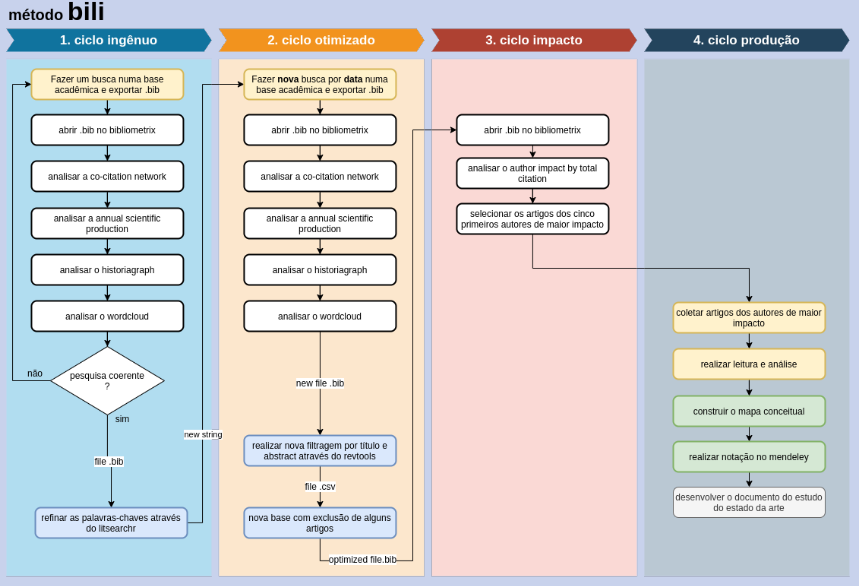
\includegraphics[width=\textwidth]{metodo_bili.png}
    \caption{Three simple graphs}
    \label{fig:three graphs}
\end{figure}
%----------------------------------------------------------